\chapter {Resultados}
Foram analisados através de mais de 40M de loc nos projetos Ant, CommonsCollections, FreeMind, Log4j, SquirrelSql, Xerces, Checkstyle, FindBugs, Jetty, Spring, Weka.\\

\section{LambdaExpression}
A maior mudança ocorrida em Java 8 foi a introdução de expressões lambda, que tem por definição prover um bloco de código limpo e conciso para representar um interface usando uma simples expressão. Também melhoram a manipulação de \textit{collections} tornando fácil a iteração através de filtros para extração de dados e adiciona novas características de concorrência que aumenta a performance em ambientes multicores.\\

\textit{Anonymous inner classes} foram projetada para facilitar o desenvolvedor a tratar seus dados de forma fácil, mas isso não é tão simples como deveria ser, além de suas implementações serem usadas somente em local específico da aplicação, em boa parte de seu uso para tratar eventos decorrentes do usuário ou de algum processamento específico. Expressões Lambda podem vir a substituir \textit{Anonymous inner classes} o que acarreta em uma redução de linha de código e de tipos utilizados no sistema.\\

Dentre os projetos analisados foram encontrados ocorrências de tal característica, \textit{Lambda Expression}, somente nos projetos \textit{Checkstyle} e \textit{Spring}, 320 e 420 ocorrências respectivamente totalizando 752 ocorrências dentre um total de XXX nós analisados.\\

Tendo em vista que expressões lambdas podem vir a substituir \textit{Anonymous inner classes} e reduzir o número de \textit{types} dos projetos. Foram encontradas nos projetos CheckStyle e Spring, 2376 e 113069 ocorrências respectivamente de \textit{Anonymous inner classes}. Com uso de expressões lambda a quantidade de ocorrências de \textit{Anonymous inner classes} e \textit{types} teria a tendência natural de diminuir seu uso.\\

Um uso corriqueiro de expressão lambda seria para substituir o seguinte bloco do projeto Checkstyle:
\begin{lstlisting}
	//Without Lambda Lambda Expression
	button.addActionListener(new ActionListener(){
		public void actionPerformed(ActionEvent e) {
			System.out.println("button clicked");
		}
	});


	//With Lambda Lambda Expression
	button.addActionListener(event -> System.out.println("button clicked"));
	
\end{lstlisting}

Isso acarretaria diminuição no uso de \textit{Anonymous inner classes} para uma forma mais atual e nesse simples exemplo seria um redução de 80\% sobre o código utilizado anteriormente. E ainda uma redução de tipos 3 tipos(ActionListener, ActionEvent e void) para um único método anônimo que acarreta em 300\% na redução de tipos.




\section{ANT}
Até a última versão deste projeto, 1.9.5, não foram encontradas utilização métodos com \textit{vargs}, expressões lambdas, \textit{switch} com \textit{strings} e nem \textit{try} com \textit{resources}.\\

Este projeto faz um bom uso de tratamento de exceções sendo encontrado em toda história de desenvolvimento foram produzidas 28 versões deste e com um total de 34722 blocos \textit{trys}, onde em média foram encontradas 1240 destes blocos por versão. E deste total pode-se verificar um total de 513 ocorrências de blocos \textit{trys} com \textit{catchs} iguais totalizando em 1,5\% de código repetido neste quesito conforme ilustra Figura: \ref{fig:TrysAnt}.\\

	\begin{figure}[h]
		\center
		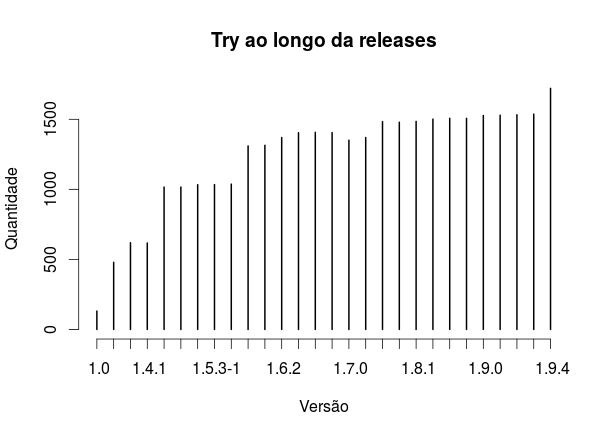
\includegraphics[width=0.7\textwidth]{Imagens/trysAnt}
		\label{fig:TrysAnt}
		\caption{Tratamento de exceção ao longo das releases.}
	\end{figure}

Entretanto pode-se constatar conforme ilustrado na Figura: \ref{fig:catchIguais} que em todas as versões do projeto \textit{ANT} possui o tratamento de exceção como blocos \textit{catchs} iguais sendo contabilizado um total de 513 ocorrências e dando atenção especial entre as versões 1.9.0 e 1.9.5. Entretanto a partir da versão 1.9.0 por volta de 2012, java possuía o mecanismo de \textit{multicatch} que fora lançado por volta de 2011 em java 7. Entre as \textit{releases} desta versão foram encontradas em cada um dos 5 lançamentos do \textit{ANT} por volta de 27 ocorrências iguais de \textit{catchs} e acarreta em um total de 135 blocos repetidos. Caso fosse adotado \textit{multicatch} seria reduzido somente a 5 blocos a cada versão existente o que seria uma redução de código repetido em aproximadamente 18\%, e isso acarretaria em um código mais atual e elegante.\\

	\begin{figure}[h]
		\center
		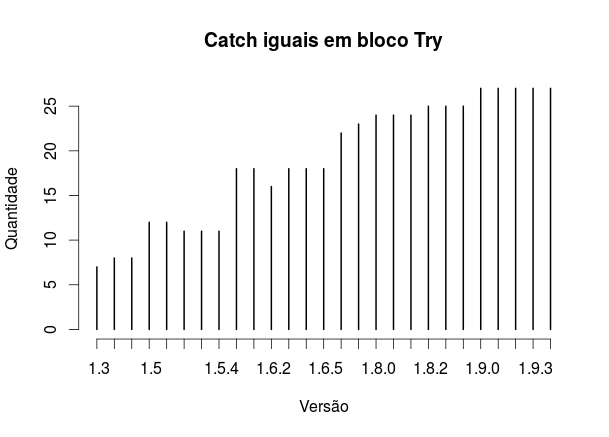
\includegraphics[width=0.7\textwidth]{Imagens/catchsIguais}
		\label{fig:catchIguais}
		\caption{Bloco Try com catchs iguais ao longo das releases.}
	\end{figure}
